%
% File: chap01.tex
% Author: Liam O'Shea
% Description: Introduction chapter where the boxing goes.
%
\let\textcircled=\pgftextcircled
\chapter{Background \& Research}
\label{chap:intro}

\initial{T}his chapter describes and explains boxing concepts which are important to understanding the goal of the project. It gives an overview of the types of punches a boxer must execute along with common errors associated with those. It also reviews relevant literature in areas covered by this thesis and explores the current cutting edge possibilities.
%=======
\section{Boxing Background}
\label{sec:sec01}
Boxing requires an incredible amount of co-ordination and timing as well as the ability to rapidly execute punches in a controlled and precise manner. Unlike professional boxing which is 12 x 3 minute rounds an amateur bout is 3 x 2 minute rounds which changes the dynamics of the contest. Amateur boxing relies on a points scoring system since there is often insufficient time for knockouts, requiring amateur boxers to rely on the mastery of technique and proper form. For example dropping a guard for a split second can open you up to an experienced boxer and could spell disaster.

As someone who has boxed for over 5 years and captain of the University of Bristol's Amateur Boxing Club (UOBABC) I understand the difficulties of developing good technique and how much time and experience is required from a coach to develop a new boxer. This one-on-one time is incredibly valuable but also expensive and for the large majority very hard to get. ZerotoHero aim is to be able to identify different types of punches and to offer feedback on the quality of the movement. This will bring some much needed expert advice to a beginner who can practice in the comfort of their own home.

I am using my own experience and that of local professionals, coaches and local legend Denis Stinchcombe MBE the centre director of Riverside Youth Project and Registrar for the Western Counties for the Amateur Boxing Association.
 

\subsection{Motivation}
\label{subsec:subsec01}
This research is borne out of a desire to improve access and cost to boxing coaching which are problems I have encountered first hand through the University Boxing Club. In a wider context it could be used in developing countries where physical access to coaches with the required expertise may be difficult as well as local clubs in the UK.
Every year UOBABC takes in new members that are total beginners. We spend an enormous amount of time and effort helping them learn the basics and encourage people to practice at home. The problem from a boxers perspective is that it is incredibly hard to spot your own faults, especially without experience.
If it was possible to practice at home with the benefits of coaching it would bring massive improvements to a trainees ability. The current most effective way to train as an individual is to stand in front of a mirror and observe yourself while shadow boxing.
It could also be used as a way to introduce younger children to the sport since the Kinect is incredibly popular in that demographic and so 
is a good choice from an inclusion perspective.
\section{Boxing Technique}
\label{sec:sec02}
For the scope of this project I am going to focus on the most common orthodox stance. There are tens of slight variations on each punch but I am going to focus on the core foundations and important principles from which these can be built.
\subsection{Stance}
\label{subsec:subsec02}
The most fundamental building block of boxing is the stance, that is how you hold and position your body as well as the placement \& orientation of your feet. A good stance is crucial since it allows the boxer to be well balanced and light on their feet, allowing fast movement in any direction as well as the ability to quickly duck, weave, slip and bob and lay back to avoid punches. It is also crucial for offence since the power from punches come from the transfer of weight from one leg to another which requires a very specific twisting hip movement. Often beginners forget this crucial step and so I'm hoping to use this unique trait to help me judge quality later on. A successful stance should have the following characteristics:

\begin{itemize}
  \item Left foot forward, right foot back with a distance slightly wider than shoulder width with a 45 degree angle twist.
  \item Right heel of the ground at all times with weight distribution mostly on your back leg.
  \item Chin tucked down.
  \item Right hand on the right hand side of your chin, left hand should be a few inches in front of the left side of the face.
  \item Elbows tucked in to protect the torso section.
  \ldots
\end{itemize}

\subsection{Punches}
\label{subsec:subsec03}
\paragraph{Jab}
The elbow should stay tucked in while the left fist extends with palms facing inwards before twisting your wrist at the last moment. The natural thing to do is extend the punch with palms facing down, unfortunately this immediately makes the elbow stick out which allows the opponent to easily see you are about to throw a punch (telegraphing) while opening up your body for a counter attack. The punch should also finish so your arm is fully extended which helps to extend your reach and protect your chin before speedily returning it to the guard position.\newline
Target Characteristic: Elbow movement

\paragraph{Cross}
The cross is designed as your heavy straight punch and as such is slower but more powerful. To get a snappy and powerful punch it is important to transfer your weight rapidly from your back leg to your front leg, twisting your hips.\newline Target Characteristic: Twisting of the hip\newline
Target Characteristic: Distribution of weight to the front foot


\paragraph{Hooks}
Your elbow should be raised to shoulder height and your fist and shoulder should be at 90 degrees to each other. A transfer of weight between the front foot and back with the twisting of the hip is essential.\newline
Target Characteristic: Elbow being raised to parallel\newline
Target Characteristic: Hip twist resulting in weight transfer from front to back\newline

\paragraph{Uppercuts}
This required the fighter to crouch down into the squat position and throw a punch vertically upwards, with the aim of striking the opponent's chin.
Target Characteristic: Sufficient crouching before releasing the punch\newline
Target Characteristic: Directly vertical punch, keeping guard close at all times.\newline

\section{Kinect}
This section provides some background information about Microsoft Kinect that is important for understanding the features and limitations of Kinect Analysis. According to Microsoft, the Kinect  has worldwide sales of approximately 28 million units and contains an RGB camera, an infrared (IR) emitter and an IR depth sensor as well as a multi-array microphone. The interaction space of the Kinect is limited by the field of view of the Kinect cameras. The Kinect has a 43\degree vertical by 57\degree horizontal field of view. The Kinect sensor can be tilted using a built-in tilt motor. Tilting the Kinect increases the interaction space by $+27$ and $-27$ degrees.
The Kinect sensor provides sensor data in form of data streams. It can capture audio, color and depth data. In addition, it can process the depth data to generate skeleton data. Therefore, the Kinect offers four different data streams that can be accessed: audio stream, colour stream, depth stream and skeleton stream. The streams can deliver at most 30 frames per second (FPS) using a resolution of $640\times480$ which drops to 12 FPS with a resolution of $1280\times960$.

\begin{figure}[h]
\centering
\begin{minipage}{7.0cm}
    \centering
    \subtop[]{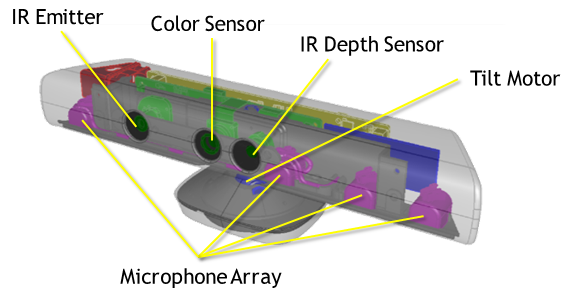
\includegraphics[height=0.15\textheight]{fig02/kinect}}
    \label{fig:1}
\end{minipage}
\begin{minipage}{7.0cm}
    \centering
    \subtop[]{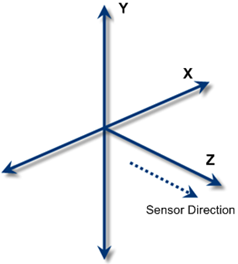
\includegraphics[height=0.15\textheight]{fig02/xyz}}
    \label{fig:2}
\end{minipage}
\mycaption[ALLData] {(a) Kinect 
(b) Kinect Dimensions}
\end{figure}


\begin{figure}[h]
    \centering
    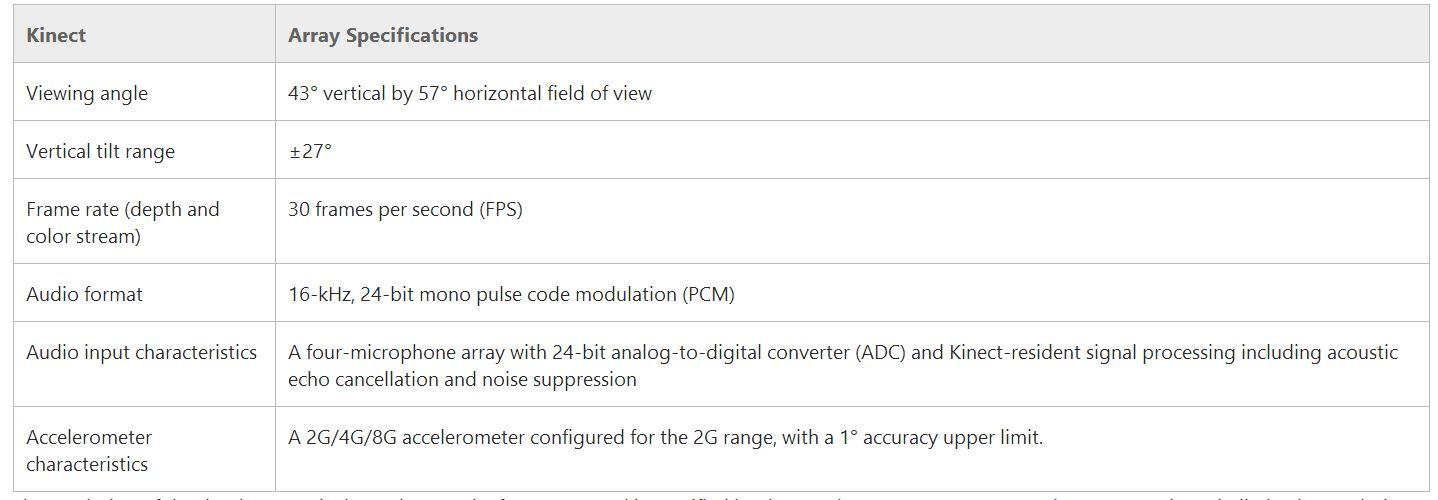
\includegraphics[height=0.25\textheight]{fig02/kinspecs.jpg}
    \mycaption[Kin Specs]{Kinect Specifications}
    \label{fig:kinect}
\end{figure}
\begin{figure}[h]
    \centering
    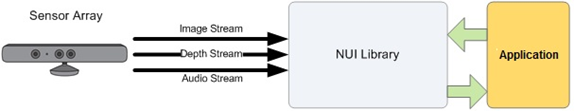
\includegraphics[height=0.15\textheight]{fig02/pipeline}
    \mycaption[Kin Specs]{Kinect Specifications}
    \label{fig:kinect}
\end{figure}

\paragraph{Depth \& Infrared Stream}
The depth sensor generates invisible IR light to determine an object's depth from the sensor. The primary use for the IR stream is to improve external camera calibration using a test pattern observed from both the RGB and IR camera to more accurately determine how to map coordinates from one camera space to another. \cite{irstream} The NUI API uses the depth stream to detect the presence of humans in front of the sensor.\cite{winSDK} Skeletal tracking is optimized to recognize users facing the Kinect, so sideways poses provide some challenges because parts of the body are not visible to the sensor.

\begin{figure}[h]
    \centering
    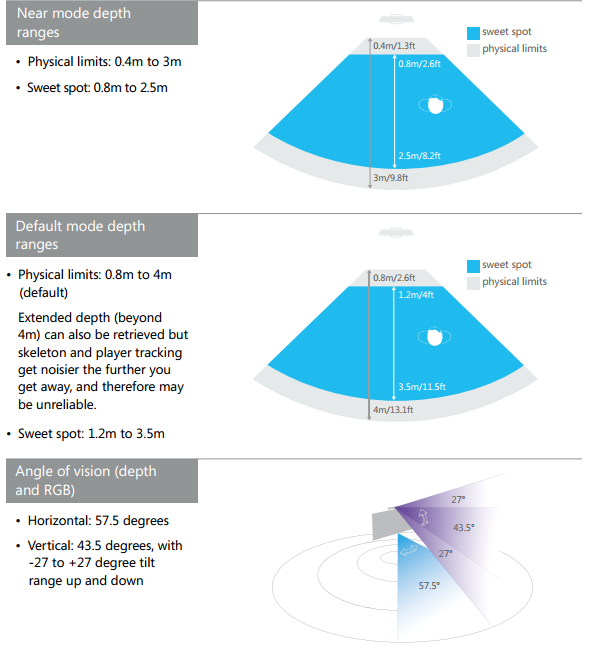
\includegraphics[height=0.45\textheight]{fig02/kinDepth}
    \mycaption[Kinect Depth Specifications]{Kinect Depth Specifications.}
    \label{fig:kinsdepth}
\end{figure}


\subsection{Skeleton \& Joint Tracking}
The Kinects default tracking mode can track up to 20 joints per skeleton providing the subject is standing relatively face on and are fully visible to the sensor. Although the Kinect is capable of different modes (e.g. sitting) this is not relevant in the context of my project.
Each skeleton frame contains the position of each joint as well as information about the tracking quality. Joints can have one of three different tracking states,  Not Tracked (0), Inferred (1) and Tracked (2), this flag is useful as an indicator of the quality of the measurements you are receiving for a particular joint. When possible, tracked joints are used to help calculate the position of those joints that cannot be directly tracked hence the ability to infer joints. The Kinects default tracking mode is designed to track people who are standing and fully visible to the sensor. The default range requires skeletons to be at least 80 centimetres away from the device to be tracked properly.

\begin{figure}[h]
    \centering
    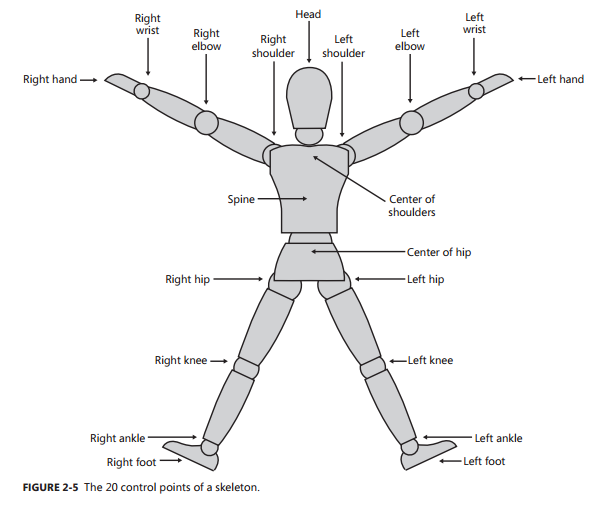
\includegraphics[height=0.40\textheight]{fig02/kinSkel}
    \mycaption[Kinect Joint Tracking Skeleton]{Kinect Joint Tracking Skeleton.}
    \label{fig:kinskel}
\end{figure}



\section{Literature Review}
The Kinect is currently a rich area of research in its own right and it straddles the fields of Image Processing and Computer Vision as well as Human computer Interaction which are exciting and popular areas of research. I wanted to see what was capable with the Kinect at the cutting edge of research so I consulted the most recent papers from the Conference on Computer Vision and Pattern Recognition (CVPR), International Conference on Computer Vision (ICCV) \& European Conference on Computer Vision (ECCV) to find the most relevant and useful research.
In 2013 a controlled study of 16 people who were blind or who had low vision was ran to test the usefulness of Eyes-Free Yoga: An Exergame Using Depth Cameras for Blind \& Low Vision Exercise. The purpose of this was to teach the participants yoga poses using audio feedback and a positive response from participants.\cite{Rector2013} The study took the Kinect joint positions and calculated joint angles while using heuristics for each pose. However the study only measured success using 6 unique static poses that were required to be held for an extended period of time. In contrast boxing requires fast repeated movements with many of the movements sharing similarities which make them harder to differentiate. Therefore I did not find this useful for evaluation the feasibility of my project.

The Kinect has also been used to evaluate a dancers performance with comparison to a professional dancer in real-time\cite{Alexiadis2011}. A score was achieved by adding three different metrics, one from the correlation coefficient of quaternions, another using joint velocities and finally a `'3D flow Error,'' calculated from frame vectors.\newline
The experimental results were encouraging with most of the scores consistent with real-life rankings with the exception of a few poor results due to bad skeleton calibration and tracking. This work draws strong parallels in what I am trying to achieve and demonstrated that the Kinect was a viable option for my work.

Other work such as disc throwing performance\cite{Yamaoka2013} also showed some promise with limited success with the lower ability groups improving their movement. This approach simply used joint angles to measure 5 different phrases of the throw and compare that to joint angle rules. I found this to be overly simplistic in comparison to the project I am trying to achieve although it did indicate that joint angles may be a useful technique for judging movements.



Recognising punches is an example of activity recognition in which there has been a fairly large body of work using the Kinect since it was released to PC in 2012 by Microsoft. 

BLAH BLAH BLAH did this. Good for this, bad for this.



















\section{Existing Products}
\par{UFC Personal Trainer}
The closest commercial product is `UFC Personal Trainer' a very broad commercial Xbox game aimed at introducing people to UFC. After evaluating this product it became clear to me that it’s main focus is  exercise regimes rather than technical fighting. Therefore it does not offer the preciseness or technical fighting focus that I require. In this game you technically wrong punches will still register and several movements are unrealistic.

\paragraph{Kinect sports boxing game}
This game has very poor punch discrimination and does not require any sort of real boxing ability. The goal here is usually to punch towards the Kinect controller as quickly as possible. It fails to recognise properly thrown hooks and uppercuts and translate those into the game. 

\paragraph{Fighers Uncaged}
This game has generally poor reviews from reviewers, with most complaints involving the reliability of the Kinect to accurately measure fighting moves. \cite{gamerev1} `'When the fights actually start, pulling off moves becomes a series of desperate flails, trying to get the game to recognize your actions.''\cite{gamerev2} 
and `'The game fails to register most of the movements'', `'The idea was great for Kinect, but something went horribly wrong along the way. Kinect is supposed to register your every kick and punch, but it only catches about the half of them.'', `'the Kinect control is lazily implemented.''\cite{gamerev3} \newline

\paragraph{Literature \& Product Conclusion}
From my research and product comparisons I concluded that the Kinect was a viable option for my project and worth pursing. Crucially however there has been no research specifically into the area of boxing with the Kinect which brings it's own unique challenges. Boxers are trained to be fast, well guarded and to give very little away in their movements, especially punches. Therefore many of the punches and poses are very similar since the goal is to be naturally evasive. This will make segmenting punches and giving useful quality metrics challenging in it's own way unlike say a discus throw. A boxers stance is often quite `closed' so I anticipate challenges tracking obscured joints and the overall accuracy of inferred joint positions. However I could see from the above studies that hip movement could be effectively tracked which was my main concern when evaluating the Kinect since all boxing moves rely on the hip rotation.
\newline\newline 
It is clear that this will not be an easy project. Many years of Microsoft research have gone into the current Kinect but surprisingly games for their flagship console fail to provide tracking accuracy that satisfies consumers. Furthermore no commercial products exist that incorporates proper boxing technique into a game, suggesting there may be limitations with the hardware that prevent this or that it it simple difficult to do. However the research in this area has shown sufficient promise for me to combine my boxing and computer science knowledge to work on this problem.
%=========================================================

